\part{Fondements théoriques du traitement des archives numériques d’exposition}

\chapter{La diplomatique de l'archive d'exposition et son cycle de vie}

La situation de crise documentaire évoquée dans le chapitre précédent fait remonter plusieurs problématiques ayant une incidence sur la gestion documentaire, à l'instar de la perte de l'information. Dans un tel environnement, l'information ne se perd pas seulement à cause d'un mauvais rangement des fichiers. Cela est également lié à des réflexes quotidiens des salariés tels que la copie des fichiers des espaces de stockage individuels vers les espaces partagés, leur déplacement d'une arborescence à une autre,  réflexes souvent perçus sans risque au premier abord. Pour remédier à cette situation, Luciana Duranti présente dans son article sur \textit{\enquote{la diplomatique des documents électroniques}} que la diplomatique est la science fondamentale qui détermine les caractéristiques extrinsèques  et intrinsèques des documents. Son étude prend appui sur les documents numériques\footnote{\cite{duranti-2003}}.

L'analyse de ces propriétés exige de mettre l'accent sur le statut profond du document. Ce qui impose une analyse rigoureuse des caractéristiques intrinsèques des documents :  sa nature, son authenticité et son contexte de production. En effet, cette approche fondée sur trois composantes est ce qui donne du sens à la transformation d'un vrac numérique passif en un fonds exploitable et sécurisé. Elle se décline en plusieurs articulations : la première approche se concentre sur la typologie documentaire et la valeur administrative; la deuxième sur les conditions d'altération et la sur la valeur probante des documents; la troisième met en avant les liens organiques entre les documents et les activités qui les génèrent. 

Cette approche diplomatique trouve une limite d'application dans le contexte du MAD, du fait de plusieurs facteurs : l'absence de charte documentaire ou éditorial :  aucun document d'une même typologie ne se ressemble, ni ne possède la même structure interne.

Le présent chapitre s’appuie sur ce cadre théorique et se propose de faire une étude fine : sur la nature et les valeurs de l'archive d'exposition, son évolution au fil du temps, avant de se concentrer sur les moyens de restitution du contexte face à une désorganisation.


\section{Nature juridique et historique d’une archive d'exposition}

 \textit{\enquote{La problématique des archives des musées en France se révèle aujourd’hui particulièrement complexe à appréhender pour les professionnels du patrimoine}\footnote{\cite{sasseti-aguilera-2020}. p. 227.}}.
 \textit{Véronique Sassetti-Aguilera}
 
 
La place des archives au sein des musées est une question brûlante. Elles répondent aux besoins à la fois ponctuels et historiques des organisations. Pour les comprendre, il faut être en mesure de déterminer leur nature, leur valeur et la manière dont elles évoluent dans le temps.


\subsection*{Une archive composite et plurielle}

À la différence d'autres séries documentaires produites dans les musées telles que les dossiers du personnel, les dossiers des marchés où les procès verbaux du conseil d’administration; les archives d'exposition se distinguent par leur caractère transversal. Elles constituent la production cloisonnée et interactive d'un ensemble de producteurs. 

En effet, elles sont appréhendées comme une construction collective dont la cohérence ne repose pas sur l'unité de son producteur mais sur l'unité du projet d'exposition. Les archives d'exposition sont le fruit d'un ensemble complexe. Ce qui donne du sens à cet ensemble c'est l'activité productrice, le projet d'exposition. Cette perception permet de rallier les archives à tout ensemble de logiques. Elles s'inscrivent dans la logique :  administrative, en ce sens ou elle émane d'un projet; scientifique, car elles résultent d'une réflexion et d'échanges autour des œuvres muséale,  parce qu'elles sont le produit d'une activité de conception exposition ;  et communicationnelle, par les documents de la médiation et de diffusion des expositions.

\subsection*{La valeur de preuve et de mémoire}

Selon Théodore Schellenberg, les documents publics modernes disposent de deux types de valeurs : la valeur primaire (c'est celle qui est utile à l'organisme pour les besoins de preuve, notamment financières, juridiques, administratives ou opérationnels), et la valeur secondaire (utile à d'autres organismes ou au public une fois que le document n'est plus utilisé au quotidien)\footnote{\cite{schellenberg-appraisal-1956}. p. 6-7. }. L'auteur s'appuie sur l'utilité de façon durable des archives dans les institutions publiques pour mûrir sa réflexion. Dans la valeur secondaire, il identifie la valeur probante comme étant ce que prouve le document sur l'organisation, les fonctions et le fonctionnement de l'organisme qui l'a produit\footnote{\cite{schellenberg-appraisal-1956}. p. 6-7. }. En d'autres termes, l'archive remplit une fonction de preuve dans le cadre de l'activité ponctuelle d'un organisme à travers sa valeur primaire. Elle documente et témoigne de l'organisation, du fonctionnement et des actions de l’institution dans la durée, en vertu de sa valeur probante. Au-delà de cet aspect, l'archive est la mémoire de l'institution, puisqu'à travers ses documents, elle peut retracer sont histoire depuis la genèse.

Dans le contexte de l'exposition, l'archive prouve, une fois l'exposition terminée, comment le musée à fonctionné pour réaliser ce type de projets : elle retrace le processus institutionnel qui a permis de produire l'exposition (les décisions prises, les procédures, les acteurs et leurs responsabilités). Ces informations, portant sur des décennies, et qui concernent plusieurs expositions, constituent la mémoire organisationnelle et présentent un intérêt pour les agents, en premier lieu, et pour les chercheurs, dans un second temps. Cet intérêt en deux temps se recoupe avec les écrits de Schellenberg : les agents s’intéressent à la valeur primaire tandis que les chercheurs cultivent leur intérêt pour la valeur secondaire, la valeur probante. 

\section{Application du cycle de vie des documents au contexte numérique du MAD}

Le cycle de vie est appréhendé comme l'ensemble des étapes de l'existence d'un document de sa création à la mise œuvre de son sort final\footnote{\cite{kern-holgado-cottin-2015}.}. Dans la conception archivistique, Yves Pérotin fait une présentation de la \enquote{théorie des trois âges}, dans son article sur \textit{L'administration et les \enquote{trois âges} des Archives}. Selon lui, les trois moments de la vie d'un document sont : l'âge administratif, l'âge de pré-archivage et des dépôts intermédiaires, pour finir avec l'âge de l'archivage\footnote{\cite{perotin-administration-1961}}.

Le modèle cible envisagé par le MAD pour structurer ces trois âges, à travers les différents choix d'archivage numérique possible à chaque étape du cible de vie, est présenté en annexe\footnote{Voir annexe ~\ref{annexe:choix-archivage}}. 


\subsection{Création, utilisation et circulation du document}


Les documents sont produits par les agents qui se mobilisent autour d'une exposition, en particulier le service de la production des expositions, et les conservateurs. Dans le cas d'archives numériques, ceux-ci sont conservés sur deux ensembles de stockage : les stockages locaux (serveurx, Bureau, Mes documents, téléchargement, etc.) et dans le cloud Microsoft (Equipe Teams/SharePoint, OneDrive, ainsi qu'Outlook)\footnote{\cite{dion-choix-archivage-2026}. p. 1.}. Les documents sont manipulés, modifiés et échangés justifiant leur utilisation courante : ils circulent sous formes de pièces jointes ou lien de partage par échanges de mails. Les différentes versions détenues par les producteurs sont également partagées via les plateformes de collaboration. 

Cette phase de circulation active d'un document prend fin lorsque le document n'est plus utilisé pour le travail courant, généralement à la fin d'une exposition. Ce processus amorce le passage vers la phase intermédiaire.



\subsection*{Du document courant à l’archive intermédiaire}


Arrivé à la fin de son utilité quotidienne, le document n'est pas archivé automatiquement. Pour qu'il le soit, il faut qu'il passe par la phase intermédiaire. Au cours de cette dernière, il peut être consulté pour des besoins ponctuels ou administratifs, par l'archiviste et par les collaborateurs, et conservé pendant sa durée d'utilité administrative. Dans le cas d'espèce, le basculement de la phase courant à la phase intermédiaire se décline en plusieurs articulations : 

\begin{itemize}[label=---]
	\item \textbf{Cas1}: S'il n'a pas les droits, le service informatique donne accès à l'archiviste après traitement du producteur.
	\item \textbf{Cas2}: Le producteur effectue lui-même le versement manuel sur l'espace dédié.
	\item \textbf{Cas3}: Le service informatique effectue un transfert manuel via la sauvegarde, notamment en cas d'urgence ou de départ d'un salarié.
	\item \textbf{Cas4}: Le producteur donne l'accès à l'archiviste, qui effectue lui-même une synchronisation manuelle\footnote{\cite{dion-choix-archivage-2026}. p. 1.}.

\end{itemize}

Ces situations sont pour la plupart le résultat d'une activité manuelle, exécutée soit par les intervenants directs d'un projet, soit par les personnes extérieures (l'une importante pour le bon déroulement du processus d'archivage, et l'autre pour la gestion et le suivi des activités techniques informatiques). Un cinquième scénario est envisagé si le Système Archivage électronique implémenté au sein de l'institution : le versement avec connecteur ou API (\textit{Application Programming Interface}). Il s'agit d'un recours automatisé à partir duquel les documents sont transférés automatiquement des espaces de stockage du producteur vers l'espace de dépôt des versements. L'API est la passerelle qui permet à deux logiciels de dialoguer entre eux\footnote{\cite{orange-api-2025}.}.

Quatre solutions d'archivage intermédiaire sont identifiées : le stockage sur serveur sécurisé et sauvegardé (YODA), un pan intermédiaire mutualisé (VaS), un externalisé sous agrément du service interministériel des archives de France et un interne (VITAM). La première représente la situation actuelle du MAD.


\subsection*{Le sort finale }

Parler du sort final d'un document revient à expliquer les moyens mis en œuvre pour assurer sa conservation définitive. En d'autre termes, il s'agit des processus qui concourent à ce que l'information soit conservée dans des conditions optimales afin de garantir son accès dans le temps. L'institution française en charge de la conservation des archives définitives des institutions patrimoniales comme le MAD est : les Archives nationales. Le versement est prévu à \enquote{l’échéance de la durée d’utilité administrative (DUA)des documents. Dans le cas des archives d’exposition, la DUA est de 10 ans à compter de la clôture du dossier d’exposition l’exposition environ 1 an après le démontage}\footcite[version 2, p.~4]{bomel-dion-note-cadrage}. Pour des besoins de conformité et de sécurité, l'information est transférée, de l'organisme vers le logiciel VITAM des Archives nationales repose. Ce transfert se base sur le modèle de l'OAIS (\textit{Open Archival Information System}), notamment à travers la conception d'un SIP (\textit{Submission Information Package}) : c'est le paquet d'archivage à verser. Sa structure et toutes les informations relatives au versement sont décrites dans un manifeste conforme au standard d'échange des données pour l'archivage (SEDA). 

\section{ Le plan de classement comme instrument de validation intellectuelle}

En archivistique, il existe plusieurs outils pour comprendre et faciliter la recherche et l'accès à l'information dans les institutions. Le plan de classement est l'outil de gestion fondamental qui permet la mise en ordre physique et intellectuelle des documents. Il constitue la représentation intellectuelle de l'activité des producteurs et permet de restituer les relations qui leur donnent un sens. Placé dans l'environnement électronique, le plan de classement est soumis à des contraintes de structure tout en bénéficiant de fonctionnalités inexistantes dans les organisations papiers\footnote{\cite{collet2012}. p. 245.}. Si le classement, qu'il soit papier ou électronique se base dans les deux cas sur une structure organisée, la nature du support modifie néanmoins les pratiques de consultation. Dans le cas du papier par exemple, l'archiviste peut, par peut déplacer un dossier pour des besoins de consultation en remplaçant y un fantôme — une simple feuille pour indiquer l'absence du dossier. Dans l'environnement numérique, cette pratique n'a pas d'équivalence direct : le fichier original demeure à son emplacement, et c'est une copie qui est faite dans un environnement sécurisé pour la consultation sur place, sans jamais déplacer ni retirer le document d'origine

\subsection*{Le classement fonctionnel et le principe de provenance}

Comme nous l'avons mentionné ci-dessus, l’exposition est produite dans le cadre d’une grande collaboration interne ce qui génère un quantité importante de documents. Dans le contexte numérique, les documents produits diffèrent selon leur format et leur type : on se retrouve donc face à une hétérogénéité des documents. Or, en archivistique, la forme ou le support des document n'a pas d'importance, dès lors qu'ils sont produits ou reçus dans le cadre d'une même activité, d'un même projet, ils sont considérés comme liés à un même ensemble archivistique.\\[0.1cm]

Donc si les documents sont séparés de leur contexte initiale, il faut être en mesure de retrouver une structure qui répond à deux questions: pourquoi les documents sont produits ou reçus ? Et à qu'elle activité sont-ils rattachés? \\[0.2cm]

Dans certains cas, a structuration de l'organisme se substitue à un classement organique. Les dossiers seraient organisés par services qui les a produits (exemple : la direction \enquote{DDIP}, pour tout ce qui est produit par la Direction du développement international et de la production). Cependant, les services en raison des éventuelles réorganisations internes, des fusions de services ou de directions rendant complexe une telle mise en œuvre. 

Pour éviter cela et répondre aux questions posées plus tôt, le MAD, se résout à un classement par fonctions. Aude Collet souligne à cet égard que le plan de classement, en tant que système d'intellectuel d'organisation, structure hiérarchiquement et de façon logique les catégories descriptives conçues pour faciliter le classement et le repérage des documents\footnote{\cite{collet2012}. p. 245.}. Elle fait allusion au type de plan de classement par \enquote{activités}, car c'est lui qui facilite la compréhension du contexte de création/réception des documents au sein d'une organisation\footnote{\cite{collet2012}. p. 248.}. 

Le cadre de classement des dossiers d’exposition du MAD illustre cette logique : il est repartit en onze grandes rubriques (Propos/ Concept, Gestion des ressources, Gestion des œuvres, Mise en espace, Sécurité, Communication, Animations, Publication, Fréquentation, Bilan, Itinérance), chacune d'elle représente une activité constitutive d'une exposition\footnote{Voir annexe~\ref{annexe:referentiel-dossiers-exposition}}. 
c'est notamment la recommandation des normes et standards du records management\footnote{\cite{collet2012}. p. 248.}.

La logique d'une organisation structurée répond principalement au principe de provenance des documents. Il est compris comme le principe selon lequel chaque document doit être placé dans le fonds d'archives dont il provient et, dans ce fonds, à sa place d'origine\footnote{\cite{lodolini1995}. p. 203.}. \textit{L'Abrégé d'archivistique} dans la même lancée stipule que : \enquote{Les documents émanant d'un même producteur doivent être regroupés sans être mélangés à d'autre}\footnote{\cite{aaf-abrege-2020}. p. 137.}. Or dans la réalité du MAD, les documents relatifs à une même exposition sont aujourd'hui dispersés entre les différents services producteurs, sans regroupement systématique. Le service Archives s'attache actuellement à faire la collecte de ces documents auprès de chaque service, avec pour objectif de constituer un dossier d'exposition unique préalable aux versements d'archives définitives — ce qui nous amène, à cet égard à considérer le projet d'exposition plutôt que chaque service producteur pris isolément, comme l'unité de regroupement pertinent pour ce principe.

\subsection*{Le respect des relations entre documents, producteurs et activités}

Au-delà de sa considération d'outil d'aide au rangement, le plan de classement permet d'établir les liens entre les documents, leurs producteurs et l'activité génératrice. La compréhension de cette logique repose sur des rubriques distinctes. 

À travers la structure du plan de classement des dossiers d'exposition du MAD, on constate que l'arborescence représente les activités constitutives d'un projet d'exposition. Les documents produits ou reçus, s’insèrent dans l'une des thématiques, matérialisant le lien entre le document et l'activité. En outre, ce système permet de documenter les relations entre le document et le producteur : dans un contexte transversal où  le service de la production des expositions, la régie, les commissaires et les prestataires externes collaborent, le plan de classement centralise leurs apports au sein d'un même espace fonctionnel. Le référentiel reflète chaque étape de la collaboration, préserve l’historique de création d'un document, garantissant la compréhension du fonds.



\chapter{Les piliers scientifiques de la pérennisation numérique}

La gestion des documents numériques est un challenge auquel doit faire face toutes les institutions car, elle concerne à la fois la donnée (l'information) et le support qui la conserve. Les principaux défis sont :  conservation de  information soit conservée, son exploitabilité et son son intelligibilité dans le temps. Ces trois points caractérisent, entre autres, la pérennisation numérique. Pour se faire, il est important de mettre l'accent sur la préservation du support, de l'information qui l'entoure avant de retrouver ce que le fichier traduit grâce à l'analyse sémantique. C'est l'objectif du présent chapitre.


\section{Intégrité de la donnée et risques d'obsolescence logique}

Avant de s’intéresser au document numérique et aux conditions techniques qui permettent de le conserver et le rendre accessible, il est important de revenir sur un point : ce n'est pas parce qu'un document est stocké dans un serveur qu'il reste, pour autant, consultable dans le temps. La conservation matérielle ne dépend garantit pas son accessibilité future : celle-ci dépend de ensemble de composantes techniques (format, logiciel, environnement de lecture) — qui peuvent disparaître, changer ou devenir incompatibles avec l'environnement qui permet d'y accéder. 

\subsection*{La dépendance du document numérique à son environnement technique}

L'accès au contenu d'un document diffère selon qu'il soit sur support papier, ou numérique. Dans le premier cas, l'accès au contenu  s'effectue directement par le support. Dans le second cas, il convient de s’assurer de la  mise en œuvre moyens techniques et dispositifs afin de faciliter l'accès, la consultation et l'exploitation de l'information. L'environnement technique représente le principal moyen d'accès à l'information sur support numérique. 

Le \textit{vade-mecum} \textit{Les archives électroniques} du réseau Archives en musées, rappelle à ce titre que les archives numériques se caractérisent par l'information, le format et le support. Le terme d'information renvoie c'est le contenu que l'on souhaite partager\footnote{\cite{archives-en-musees-electroniques}. p. 8.}. Le format représente l'une des couches qui permettent de coder cette information et la rendre interprétable par un logiciel\footnote{\cite{archives-en-musees-electroniques}. p.8 .}. Or \enquote{les logiciels sont des outils qui évoluent : nouvelles versions non compatibles, abandon de certains formats.}\footnote{\cite{archives-en-musees-electroniques}. p. 8.}. Cette citation permet de soulever un fait déterminant : la relation de dépendance entre le support de l'information et le contexte technique de création d'un document. Le serveur, quant à lui, est l'espace de stockage des documents numériques, il facilite le maintien des données disponibles dans un environnement technique mais il n'y garantit pas l'accès ni la lisibilité dans un environnement futur.

Le \textit{vade-mecum} fait la distinction entre trois concepts : le stockage, la sauvegarde et l'archivage. Le stockage est identifié comme commun aux deux autres concepts. Il s’agit de la simple conservation les documents et des données enregistrés à un endroit précis sans autre action. Il pose également une question matérielle et technique : choix du format adéquat en fonction du lieu de conservation des supports \footnote{\cite{archives-en-musees-electroniques}. p. 9.}. L'archivage, lui, constitue la veille sur ledit format ainsi que son support de stockage\footnote{\cite{archives-en-musees-electroniques}. p. 9.}. En effet, l’archivage est l’ensemble des moyens mis en œuvre pour assurer l’intégrité, la pérennisation, l’authenticité, la traçabilité et la sécurité des données. Elle implique donc deux actions supplémentaires par rapport au stockage : une copie sur support d'archivage dédié (sauvegarde) et la garantie d'une lisibilité indépendamment des outils logiciels qui l'on créée\footnote{\cite{archives-en-musees-electroniques}. p. 9}. Nous pouvons matérialiser ces propos par le schéma suivant:

\begin{figure}[H]
	\centering
	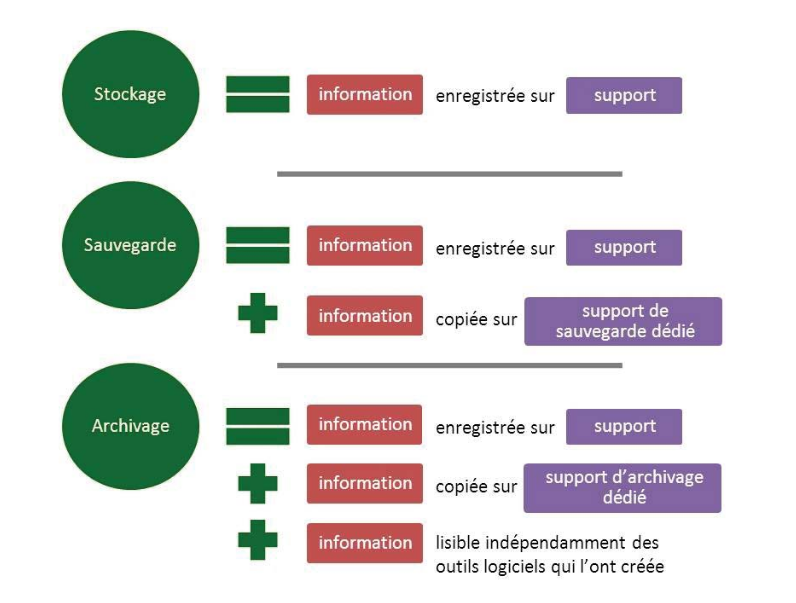
\includegraphics[width=0.8\textwidth]{Images/Archivage-et-Stockage.png}
	\caption{Distinction entre stockage, sauvegarde et archivage}
	\label{fig:Archivage-et-Stockage}
\end{figure}


Il faut avoir cette distinction en tête lorsque nous appréhendons les dossiers d'exposition stockés sur le serveur YODA. Ce dernier est un serveur de fichiers sécurisé qui fait l’objet de sauvegardes. Le fait que le serveur YODA constitue un espace de conservation intermédiaire ne signifie pas que tous les documents qui s'y trouvent sont seront lisibles et compréhensibles dans les années à venir. Cette observation renvoie à la nécessité de penser la conservation plus loin que le simple stockage du fichiers dans ledit  serveur. C’est dans ce cadre que l’archiviste a une expertise auprès du service informatique pour faire des préconisations sur la bonne gestion et conservation des documents et données. 

Cette instabilité explique pourquoi, tau MAD, la description des archives numériques se fait lors du versement à la préparation du SIP (paquet qui contient à la fois les fichiers, leurs métadonnées et un manifeste) parce que les métadonnées produites au moment de la création d'un document ne sont pas stables dans le temps. C'est le cas par exemple des documents stockés dans des serveurs partagés de type YODA. Ils peuvent être modifiés, déplacés, dupliqués, ce qui altère ce qui très souvent les métadonnées telles que la date de création, le chemin ou leurs liens avec d'autres versions auxquels ils sont liés. Ces actions créent le plus souvent des nouvelles métadonnées remplaçant les précédentes.

Cette réflexion rejoint la pensée de Luciana Duranti sur le document numérique. Elle considère que la diplomatique n'appréhende pas le document comme un contenu isolé, elle s’intéresse à la fois aux caractéristiques extrinsèques (le support, le format) et intrinsèques (contexte de création, le créateur, les actions, etc.)\footnote{\cite{duranti-2003}. p. 607.}. À partir de ces réflexions, il convent de s’interroger sur les risques liés à la conservation de ces documents.


\subsection*{Les risques liés à la conservation des documents}

Émilie Goubin identifie deux risques majeures liés à la gestion de l'information sur support numérique : \enquote{la conservation à long terme, risque lié à l'obsolescence des supports, des formats, mais aussi des organisations existantes; l'identification et la traçabilité, en lien avec [...] l'\enquote*{infobésité}et les risques juridiques}\footnote{\cite{goubin-2016}. p. 149.}. 

L'auteur aborde pas le risque lié à la conservation à long terme (l'obsolescence), d'un point de vue technique, et le subdivise en trois : 

\begin{itemize}[label=---]
	
\item{L'obsolescence des supports} : Il consiste en la fragilité physique des espaces de stockage des documents numériques, tels que les serveurs, les disques durs. 
\item{L'obsolescence des formats de fichiers} : Elle est causée par l'évolution des logiciels qui permettent de lire le format de fichier. C'est ce qui entraîne très souvent la perte de l'information\footnote{\cite{archives-en-musees-electroniques}. p. 8.}.
\item{L'obsolescence des organisations existantes} : Avec les fusions, la mutation des services, ainsi que la dématérialisation des procédures, une faille se crée au niveau de la fragilité du circuit habituel de l'information\footnote{\cite{goubin-2016}. p. 151.}. \\[0.1cm]

\end{itemize}

Le deuxième risque soulevé par Emilie Goubin, lié à la production de masse des données non structurées se caractérise par deux notions fondamentale : 

\begin{itemize}[label=---]
\item{L'infobésité} : C'est la surabondance d'information numérique présente quotidiennement et sous toutes ses formes\footnote{\cite{cigref2011risques}. p. 12.}.
\item{La perte de traçabilité}: Elle renvoie à la difficulté d'accéder au contexte de production d'une information, encore moins à son circuit dans une institution. 

\end{itemize}

Il est important de retenir que la conception archivistique, se doit de limiter les risques qui peuvent compromettre la lisibilité et l'intégrité d'un document numérique dans le temps.


\subsection*{Les principes de pérennisation}

Les besoins de pérennisation des documents après leur archivage soulèvent beaucoup de questionnements chez les archivistes, les conservateurs du patrimoine\footnote{\cite{chabin-2004}.}. Dans l'introduction de la revue consacrée au document numérique, Marie-Anne Chabin explique les raisons pour lesquelles la pérennisation est centrale aujourd'hui. Elle démontre que le nœud du problème se situe bien au de-là de la place du stockage, à ce titre, elle déclare que : \enquote{[...] c'est comment \enquote*{faire passer les années} à tous ces objets numériques [...] demain ou après-demain, pour pouvoir affirmer son droit, savoir ce qui s'est passé ou éviter de refaire ce qui a déjà été fait}\footnote{\cite{chabin-2004}.}. 

Pour garantir que les objets numérique ne perdent pas leur valeur de preuve, plusieurs moyens techniques et méthodologiques sont mobilisés. Le premier est le contrôle de l'intégrité qui permet de vérifier la cohérence de la de l'information. Le but est de vérifier que le document n'a subit aucune transformation, modification ou altération. Pour procéder à cette vérification, on peut utiliser l'empreinte numérique. La Bibliothèque nationale de France BnF la définit comme \enquote{une chaîne de caractères produite par l'analyse de données binaires (suite de 0 et de 1)}\footnote{\cite{bnf_integrite_donnees_numeriques}.}. Elle prend la forme d'un fichier ou un répertoire. Le but est de comparer les deux états d'un même objet numérique à des moments différents afin de vérifier s'il a été altéré\footnote{\cite{bnf_integrite_donnees_numeriques}.}.

Dans notre contexte de travail, cette empreinte n'est cependant pas exploitée pour des besoins de contrôle d'intégrité dans un premier temps, mais plutôt pour l'identification des doublons au sein du vrac numérique. \\[0.1cm]

Les deux autres points de la pérennisation sont le choix des formats et la migration. Pour s'assurer que les documents seront accessibles dans le temps, la décision du choix du format est importante, c'est se donner la possibilité d'accéder au contenu des fichiers dans le long terme. C'est une décision qui est propre à la volonté de chaque organisme en matière de conservation. À ce titre, en s'appuyant sur les recommandations imposée par le Référentiel général d'interopérabilité (RGI) aux administrations publiques, le MAD\footnote{\cite{bomel-dion-note-cadrage}. p. 4.} opte pour la répartition suivante : d'abord pour la bureautique, notamment, le PDF (\textit{Portable Document Format} / Archive), \textit{OPENDOCUMENT} et le TXT, ensuite pour les images telles que le PNG ou le TIFF, et éventuellement JPEG avec le moins de compression possible, et enfin pour les fichiers vidéos ou sonores les formats MPEG2, MPEG-4.\\[0.1cm]
		

Une fois le choix du format effectué, il convient de migrer les données du format actuel vers le format souhaité. Le fichier conserve ses fonctionnalités techniques de départ. La migration est appréhendée comme le passage d'un document d'un format non pérenne vers un format optimal. En d'autres termes, c'est le \enquote{transfert des données entre différents formats de données}\footnote{\cite{docuteam_formats_archivage}.}. 



\section{Métadonnées de structure et de préservation}

La conservation des documents numériques, telle que nous l’appréhendons dans cette partie se relève d’une forte une nécessité. Malgré les avantages qu'offrent les espaces de stockage informatiques, la problématique centrale de la pérennisation des informations demeure fondamentale. Après avoir abordé les opérations qui favorisent et permettent de rendre le document exploitable sur une longue période, on se demande maintenant : quelles sont les informations qu'on récupère pour atteindre l'objectif d'archivage?

Comme l’explique Émilie Goubin dans son article sur l'archivage électronique, l'archiviste, dans le contexte de l'identification des documents : \enquote{amené à identifier l'usage [...], l'identification de la mission pour laquelle un document est créé, [...]  l'usage qui peut être fait d'un document}\footnote{\cite{guyon-2023}. p. 152.}. Émilie Goubin va plus loin dans sa réflexion en mentionnant que l'identification du contexte de production d'un document numérique est un impératif pour la pérennité d'une archive.\footnote{\cite{guyon-2023}. p. 152.}. 

\subsection*{Identifier et décrire le document numérique}

Au-delà du nommage, chaque document dispose de propriétés techniques invisibles au premier abord, à l'instar de sa taille, son format, de sa date de création, ainsi que de ses dates de modifications. Ces métadonnées permettent de dresser la carte d'identité du document. En milieu patrimonial, d'après la Bibliothèque nationale de France (BnF), le document numérique est décrit par un identifiant unique et par un ensemble de métadonnées quelle subdivise en  trois grandes catégories \footnote{\cite{bnf-document-numerique-metadonnees}.}:


\textbf{Les métadonnées descriptives} : Il s'agit d'informations qui permettent de faire correspondre un document tant à son original ou qu'à ses différentes versions\footnote{\cite{bnf-document-numerique-metadonnees}}. Elles jouent le rôle d'identificateurs du document, puisqu’elles permettent d'identifier le son titre, son auteur, sa date de création et lien entre le documents et ses différentes versions.

\textbf{Les métadonnées de structure} : La BnF mentionne qu'il s'agit de, \enquote{rattacher les fichiers d'un même document entre eux, de restituer la structure du document: de connaître tous les fichier qui composent un document [...]; connaître la relation physique entre ces fichiers}\footnote{\cite{bnf-document-numerique-metadonnees}}.

\textbf{Les métadonnées administratives} : Elles garantissent la gouvernance constante de l'information. Elles répertorient les droits d'accès, notamment les droits d'auteur. Ces derniers comprennent les droits de confidentialité et les droits d'usage à savoir, la reproduction et la modification\footnote{\cite{bnf-document-numerique-metadonnees}}.
	
Cette classification n'est pas une simple théorie, elle correspond à des sections identifiées dans un format d'encodage réel et largement utilisé dans les institutions patrimoniales. Le standard METS (\textit{Metadata Encoding Transmission Standard}) utilisé pour décrire un document numérique à partir des métadonnées précise sur lui, il favorise son échange, sa gestion et sa préservation\footnote{\cite{bnf_mets}.}. Il se décompose en plusieurs sections dont; celle relative aux métadonnées descriptives (\texttt{descriptive metadata section/dmdSec} ), aux métadonnées administratives (\textit{administrative metadata section/amdSec}), et celle relative à la carte structurelle (\textit{structural map/StructMap}) , elle permet d'organiser la structure logique du document à partir de la liste des fichiers identifiés au niveau de section\texttt{file section/filSec} \footnote{\cite{bnf-document-numerique-metadonnees}}.\\[0.1cm]

Dans notre cas, contrairement à un document numérique constitué selon le standard METS, le vrac numérique se présente sous la forme d'une arborescence dépourvue d'encodage explicite. Pour étudier, on peut tout de même identifier la structural map comme l'arborescence ou la profondeur des dossiers (à titre d'exemple : \texttt{/Gestion-des-oeuvres/\allowbreak Pret/\allowbreak Dossier-Preteur/\allowbreak Fiche-de-pret.pdf}) en nous appuyant sur les outils d'archivistiques que nous évoquons à la troisième partie. Grâce à eux, on retrouve soit des métadonnées descriptives, des métadonnées administratives ou des métadonnées techniques.



\subsection*{Préserver le contexte et les relations documentaires}

Comme les autres types de documents, le document d'exposition ne constitue pas un objet isolé. Il est rattaché à un contexte précis, ici, l'exposition représente son principal contexte. À celui-ci, s'ajoute les différentes activités auxquelles il est lié, telles que la scénographie, la gestion des œuvres ou même la communication. Le document est aussi lié à la personne qui l'a produit ou reçu. Ces différentes appréhensions permettent de situer le document dans la chaîne documentaire à laquelle il appartient. La conservation des liens documentaires à aussi une grande importante dans le monde du numérique, car, comme nous l'avons mentionné dans les passages précédents, les documents se retrouvent dispersés dans plusieurs espaces de stockage. Face à cette dispersion, il est primordial de reconstituer la chaîne documentaire dont le document représente la trace. Les métadonnées constituent donc le moyens de faire remonter ces relation, en ce sens ou elles permettent d'identifier, le nom de l'auteur du document, à l'activité, ainsi que les différentes modifications effectuées sur le document.

Tout ceci nous amène à rapprocher la considération conception archivistique du document composante d'un fonds. Ses métadonnées retracent l'environnement documentaire auquel il est rattaché et mettent en évidence les liens entres les documents de cet ensemble, les opérations autours d'eux (modification, etc.).

\section{L'analyse sémantique au service de l'archivage}

Dans la pratique, l’archivage est complexe. Il convient de gérer l'information et les documents.  Cette gestion s’opère en tenant compte d’enjeux importants comme le traitement d'un ensemble éparpillé — problème fréquemment rencontré par les professionnels de l'information. L'identification de ces documents ne permet pas, à elle seule, de les gérer et d'assurer leur classement dans le fonds ou l'activité à laquelle ils sont liés. 

On se retrouve ainsi confronté à deux situations. D'abord les documents ayant les caractéristiques techniques similaires se retrouvent liés à plusieurs activités différentes. Ensuite, les documents d'une même activité ont des caractéristiques techniques similaires. 

Le classement d'un vrac va plus loin que le simple rangement des documents dans une arborescence fichiers ou alors dans un système d'archivage électronique. Face à la situation dans laquelle nous faisons face, nous nous posons la question de savoir :que représente réellement un document dans un dossier d'exposition? 
On constate qu'il implique la restitution de la fonction documentaire d'un document, ainsi que son rôle au sein d'une exposition. L'analyse sémantique apporte des éléments de réponse. 


\subsection*{Les limites d’un traitement fondé sur les caractéristiques techniques}

L'identification des caractéristiques techniques d'un document nécessite la mise en valeur des éléments tels que le format. L'écart entre la restitution du format et celui de la restitution de la fonction documentaire est considérable. Là où le premier ne fait référence qu'à l'aspect technique du document, l'autre s’intéresse à la place du document dans un ensemble. On se rend par exemple compte qu'une extension d'un fichier \enquote{.pdf}  peut renvoyer à  plusieurs catégories documentaires différentes en fonction de son contexte de création. Par exemple, un fichier .pdf qui peut très bien être un document lié au prêt des œuvres; un autre qui peut être centré sur la sécurité. Cette limite représente un enjeu pour la compréhension et la constitution d'un dossier d'exposition tel qu'il est perçu. Quelques outils d'aide au traitement archivistiques, prévus par les Archives nationales du Royaume-Uni confirment notre propos tel que l'outil qui permet de détecter les métadonnées techniques des documents\footnote{\cite{national-archives-droid}}. 



\subsection*{Le langage métier comme source d’information}

Le langage métier des producteurs constitue un élément primordial dans la reconstitution du contexte d'un document. Il favorise le traitement automatisé des documents. 

Au MAD comme la plupart des institutions, les salariés, dans l'optique de faciliter le repérage de leurs dossiers les identifient en fonction de leur vocabulaire professionnel, leur jargon. Ce vocabulaire très souvent lié à l'activité maîtresse à laquelle il est lié. Il est important en ce sens ou il permet \enquote{oui}, d'identifier l'activité, il n'est pas lié au vocabulaire informatique. 
Pour aller plus loin, il convient de préciser qu'un même sujet peut être abordé via un vocabulaire différent en fonction du métier, de ce fait on se retrouve avec un groupe de mots renvoyant à la même fonction, même utilisation ou même tâche sans que cela ne soit explicitement compréhensible. L'absence d'un thésaurus commun complique le travail de traitement archivistique et entraîne une multiplication des fichiers, voire l'apparition de doublons renommés pour faciliter la compréhension d'un corps de métier spécifique.


\chapter{L’automatisation au service du traitement archivistique}

Avec l'évolution progressive constante du métier d'archiviste et l’intégration poussée du numérique, une nouvelle approche se joue à la pratique archivistique : l'automatisation. Siham Alaoui s'interroge sur la place qu'occupe l'automatisation dans la chaîne de traitement archivistique\footnote{\cite{alaoui2024automatisation}. p. 20.}. L'auteure appuie sa réflexion sur la continuité de celle de Cook, qui lui identifie quatre paradigmes archivistiques, à savoir la preuve, la mémoire, l'identité et la communauté\footnote{\cite{alaoui2024automatisation}. p. 19-20.}. 

Face à cette évolution, l’automatisation se propose d'apporter des éléments de réponses techniques au traitement des archives numériques. En s’interrogeant sur le processus de traitement archivistique, elle vient en appuie au domaine. Avec la multiplication des supports, la quantité importante des données qui se retrouvent parfois dispersées, comme c'est le cas des données en vrac. Il devient alors difficile de repérer les informations, de les exploiter et de les mettre à la disposition des usagers. L'enjeu de ce chapitre est de s'interroger et d'identifier quels niveaux de la chaîne peuvent être automatisées tout en préservant les principes archivistiques afin d’alléger la tâche de l'archiviste.  On s’attellera à mettre en lumière l'utilisation de l'automatisation comme un levier d'amélioration et de fluidification des  traitements archivistiques. Parallèlement, on exposera les limites de ce système.

\section{Le changement d’échelle de traitement impliquant les archives numérique}

Les méthodes archivistiques restent valables dans l’environnement numérique mais leur mise en œuvre se confronte à une quantité de documents qui rend certaines opérations manuelles difficiles et chronophages. Dans le corpus étudié, on se rend compte qu'une même exposition peut se retrouver dans plusieurs répertoires, ce qui multiplie l'information.

\subsection*{Limites du traitement exclusivement manuel}

Le traitement manuel des archives est reste une opération contrôlée par l'archiviste. Il permet à l'archiviste d'être sûre de la véracité des informations recueillies et de la façon dont elles sont rangées. Toutefois ce traitement peut avoir des limites surtout face à la multiplication des supports et des données. 

Avec la masse importante de documents, le traitement des documents numériques représente une tâche fastidieuse. Plusieurs autres limites peuvent être soulevées. Sans nommage signifiant des fichiers, la gestion manuelle oblige l'ouverture individuelle et systématique des documents afin d'en identifier le contenu\footnote{\cite{chabin-vrac-2016}}. Il est à noter que cette opération peut être retardée par l'existence de conditions d'accès restrictives.


\subsection*{L’automatisation comme assistance au traitement de masse}

\begin{displayquote}
	\textit{\enquote{L'automatisation ne remplace pas l'intervention humaine\footnote{\cite{da-silva-santos-heiniger-2024}. p. 8.}}}.
\end{displayquote}
C'est ce que soulignent Sara Da Silva Santos et Fleur Heiniger. Face aux limites évoquées, l’automatisation ne se veut pas comme un outil de remplacement du traitement manuel, mais plutôt comme une aide. Celle-ci présente un réel avantage pour les archives numériques. Santos et Heiniger poursuivent en disant qu'elle\enquote{assiste la·le spécialiste dans l’identification des premiers problèmes qui créent du bruit autour des données : doublons, formats obsolètes, fichiers corrompus ou vides, etc.}\footnote{\cite{da-silva-santos-heiniger-2024}. p. 7.}. Ainsi, l'automatisation permet de réduire les délais d’exécution\footnote{\cite{da-silva-santos-heiniger-2024}. p. 6.} des tâches complexes en traitant un volume important et parfois non structurés. Un algorithme peut à la fois parcourir un ou plusieurs répertoires de fichiers, dans un temps très court, accélérant ainsi considérablement le traitement manuel qui prendrait des heures voir des jours à réaliser. Elle va plus loin en identifiant les données indésirables dans un grand ensemble, en effectuant le tri. Alaoui mentionne que l'automatisation représente une évolution du rôle de l'archiviste\footnote{\cite{alaoui2024automatisation}. p. 19-29.} en tant qu'acteur principal dans le processus. Il se retrouve dans un changement d'échelle auquel il doit s'adapter pour garantir le traitement des  documents. Cette adaptation relève d'un enjeu important étant donné que grâce à la maîtrise d'outils informatiques l'archiviste peut aujourd'hui exécuter ces tâches avec un plus de gain de temps.

Le programme présente une utilité lorsqu'il est conçu pour exécuter les tâches préalablement définies par l'humain. Ce dernier réunit un ensemble de conditions lui permettant de répondre aux exigences et à la demande du métier. Pour les archivistes, ces exigences soit à un besoin de tri, soit de classement, soit de structuration de la donnée. 



\section{De la règle archivistique à son interprétation informatique}

L'informatique est considérée aujourd'hui comme un étant un plus pour tous les domaines d'application. Les archives ne sont pas en reste. L’automatisation appliquée aux archives se subdivise en deux volets. D'un côté, le raisonnement archivistique : c'est l'idée maîtresse qui favorise la gestion documentaire. De l'autre côté, l'algorithme, qui joue le rôle de facilitateur, met en exécution de façon matérielle les règles qui sont indiquées en amont.

Dans la mesure où le programme ne sait pas en avance ce qui doit être exécuté, il ne peut pas imaginer les actions que l'humain veut mettre en œuvre. Ces règles ont besoin d’être formalisées. Cette formalisation réunit les deux notions évoquées plus haut.


\subsection*{Formaliser afin de rendre une décision automatisable}

Parler de formalisation revient à identifier l'ensemble des éléments qui permettent au programme d’exécuter des tâches et  faciliter la prise de décision\footnote{\cite{da-silva-santos-heiniger-2024}. p. 5.}. Dans le contexte archivistique,  elle nécessite d'identifier les phases qui permettent de repérer le traitement documentaire afin d’exécuter l'action à laquelle elles sont liées. C'est à cette étape que de l'archiviste se doit d'être pointilleux sur les recommandations faites. 

Comme nous l'avons mentionné plus haut, les simples caractéristiques techniques d'un fichier ne peuvent pas le décrire et le situer dans une arborescence.Il convient donc d'identifier la fonction documentaire sur la base d'autres éléments comme le nommage du fichier ou du répertoire auquel il est rattaché.C'est exactement à ce niveau qu'on peut comprendre ladite fonction.

La formalisation constitue une suite de conditions qui facilitent la mise en œuvre de ces indices. Elle permet de matérialiser différentes critères de sélection liés directement aux documents, à l'activité de laquelle ils découlent (si un document est produit ou reçu dans le cadre d'une activité de prêt par exemple), en lien avec le plan de classement. Cela ne traduit pas nécessairement le raisonnement archivistique en langage informatique, mais témoigne plutôt d'une collaboration étroite entre les deux. Il faut savoir que les règles simples et explicites favorisent la formalisation et, permettent l'exécution rapide des tâches.


\subsection*{La reproductibilité et la traçabilité des traitements}

La règle permet de rendre le traitement reproductible, de l'appliquer à un ensemble documentaire conséquent et de faire des tests appliqués à un corpus réel. Dans le traitement de masse, la reproductibilité représente un enjeu important, dans la mesure où elle permet la vérification et la comparaison des résultats d'un ou de plusieurs traitements. Sur la base de ces résultats, les professionnels disposent de la capacité de poursuivre, d'apporter des modifications ou alors de changer les règles identifiées plus haut.

Comme son nom l'indique, la traçabilité constitue l'action d'identification des opérations menées sur le corpus. Elle identifie les erreurs, les fichiers traités. Cette traçabilité peut se matérialiser lors du traitement par la génération des fichiers de logs, qui permettent de documenter chaque action algorithmique exercée sur un corpus. À partir de là, les réponses aux questions suivantes deviennent évidentes : \enquote{qui} (la personne qui a exécuté l'algorithme), \enquote{quoi} (l'objet sur lequel le traitement a lieu), \enquote{quand} (enregistre les différents moments de l'exécution), \enquote{comment} (la règle appliquée au corpus).



\section{ Les limites de l’automatisation et le maintien de l’expertise archivistique}

L'automatisation représente le moyen de faciliter le traitement de masse à grande échelle. Elle permet de standardiser les opérations archivistiques sérielles comme le tri, dont l'exécution exclusivement manuellement peut devenir difficile. Elle se heurte cependant à des limites qui rendent difficile son exécution, notamment au niveau de la prise de décision.

\subsection*{L’incertitude et les limites de la décisions}

Au regard de ce qui précède, nous pouvons dire que le programme informatique est aveugle au sens et au contexte. Là où l'outil informatique identifie les caractéristiques techniques des documents, l'humain lui interprète leur signification. Il convient de comprendre que le programme ne peut pas comprendre le contexte historique de son corpus. Les règles qu'il applique peuvent dans certains cas être incomplète de la réalité documentaire. Le programme exécute uniquement les instructions qui lui sont données. À partir de là, nous pouvons observer les limites décisionnelles que cela représente pour le traitement. Rien ne peut venir du programme informatique seul. Il ne peut pas décider les caractéristiques archivistiques à prendre en compte pour répondre aux exigences de conformité imposées par le métier.

C'est le cas dans le contexte du traitement des archives d'exposition, l'algorithme ne peut pas décider du vocabulaire qui doit être utilisé.



\subsection*{Une complémentarité entre traitement automatisé et validation humaine}

En réalité, avoir recours à l'automatisation c'est être capable de faire converger son savoir avec la compréhension informatique qui tourne derrière une machine. C'est à ce niveau qu'on remarque le travail collaboratif entre l'humain et la machine, où le traitement n’est pas purement informatique mais basé sur une vraie réflexion humaine. 
L'étude menée par Sara Da Silva Santos et Fleur Heiniger explique cette distinction. Selon leur développement, c'est l'humain qui définit en amont les règles et les lignes directives qui permettent au programme de fonctionner et comprendre les différentes tâches qu'il doit exécute\footnote{\cite{da-silva-santos-heiniger-2024}. p. 8.}. Avec du recul, l'humain est amené à penser qu'un tel recours revient à remplacer. Dans les faits, la réponse est négatives. Même si le traitement se fait de façon automatisée et que les résultats peuvent sembler conformes au traitement demandé. Un travail de contrôle humain doit être effectué, tels que le lancement de l'exécution des scripts ou la vérification de la conformité des résultats avec les besoins prédéfinis. 




